\documentclass{article}
\usepackage{geometry}
\usepackage{longtable}
\usepackage{array}

\usepackage{graphicx}
\usepackage{listings}
\usepackage{hyperref}

\lstset{
  basicstyle=\ttfamily,
  columns=fullflexible,
  breaklines=true
}

\newcommand{\modelentry}[1]{%
  \begin{figure}[h]
    \centering
    \includegraphics[width=\textwidth]{images/exported_bpmn/#1.pdf}
    \caption{Model: \detokenize{#1}}
    \label{fig:#1}
  \end{figure}
}

\AtBeginDocument{%
  \immediate\write18{./bpmn_to_image.sh}%
}

\geometry{margin=1in}

\title{MSP Report - Sprint 1}
\author{Franka Traupe, Roschanak Babai, Niklas Sander, Valeriia Baida, Guilherme Fernandes}
\date{}

\begin{document}

\maketitle

\section*{Roles}
\textbf{Scrum Master:} Franka Traupe\\
\textbf{Product Owner:} Guilherme Fernandes\\
\textbf{Quality Controller:} Niklas Sander\\
\textbf{Development Team:} Roschanak Babai, Valeriia Baida

\section*{Features}
(Proposal for sprint 2 highlighted in bold)

\subsection*{Basic Features (Implemented in prototype)}
\begin{itemize}
    \item Register account
    \item Register type of vehicle
    \item Define route
    \item Alert if speed limit is violated
    \item Calculate estimated time of arrival
\end{itemize}

\subsection*{Features from Existing System}
\begin{itemize}
    \item \textbf{Bookmarking (home, work)}
    \item Avoid tolls
    \item \textbf{Recent destinations}
    \item Show current speed (implemented already as part of speed alerts)
    \item Parking lots
    \item \textbf{Hazard reports}
    \item \textbf{Change units}
\end{itemize}

\subsection*{New Features}
\begin{itemize}
    \item \textbf{Statistics: usage and driving quality (rate of speed violations etc.)}
    \item Walking route
    \item Shared ride
\end{itemize}

\section*{Match from Features to Models}

\begin{longtable}{|>{\raggedright}p{0.4\textwidth}|>{\raggedright\arraybackslash}p{0.5\textwidth}|}
\hline
\textbf{Feature} & \textbf{Model} \\
\hline
Overall process & MyWaze.bpmn \\
\hline
Register account & MyWaze\_registerAccount.bpmn \\
\hline
Recent destinations & MyWaze\_defineDestination.bpmn \\
\hline
Define route & MyWaze\_defineRoute.bpmn, MyWaze\_calculateRoute.bpmn \\
\hline
Avoid tolls & MyWaze\_defineRoute.bpmn \\
\hline
Walking route & MyWaze\_defineRoute.bpmn \\
\hline
ETA & MyWaze\_defineRoute.bpmn \\
\hline
Current speed & MyWaze\_navigate.bpmn, MyWaze\_speedMonitoring.bpmn \\
\hline
Speed alert & MyWaze\_navigate.bpmn, MyWaze\_speedMonitoring.bpmn \\
\hline
Find parking lots & MyWaze\_navigate.bpmn, MyWaze\_defineRouteToParkingLot.bpmn, MyWaze\_calculateRoute.bpmn \\
\hline
Hazard reports & MyWaze\_navigate.bpmn, MyWaze\_reportHazard.bpmn \\
\hline
Share ride & MyWaze.bpmn, MyWaze\_registerRideOffering.bpmn, MyWaze\_arrangeSharedRide.bpmn \\
\hline
Bookmarking & MyWaze.bpmn, MyWaze\_createBookmark.bpmn \\
\hline
Statistics & MyWaze.bpmn, MyWaze\_provideStatistics.bpmn \\
\hline
Change units & MyWaze.bpmn, MyWaze\_changeUnits.bpmn \\
\hline
Register vehicle type & MyWaze.bpmn, MyWaze\_registerVehicleType.bpmn \\
\hline
\end{longtable}

\clearpage
\section*{Requirements Diagram}
\begin{figure}[h]
    \centering
    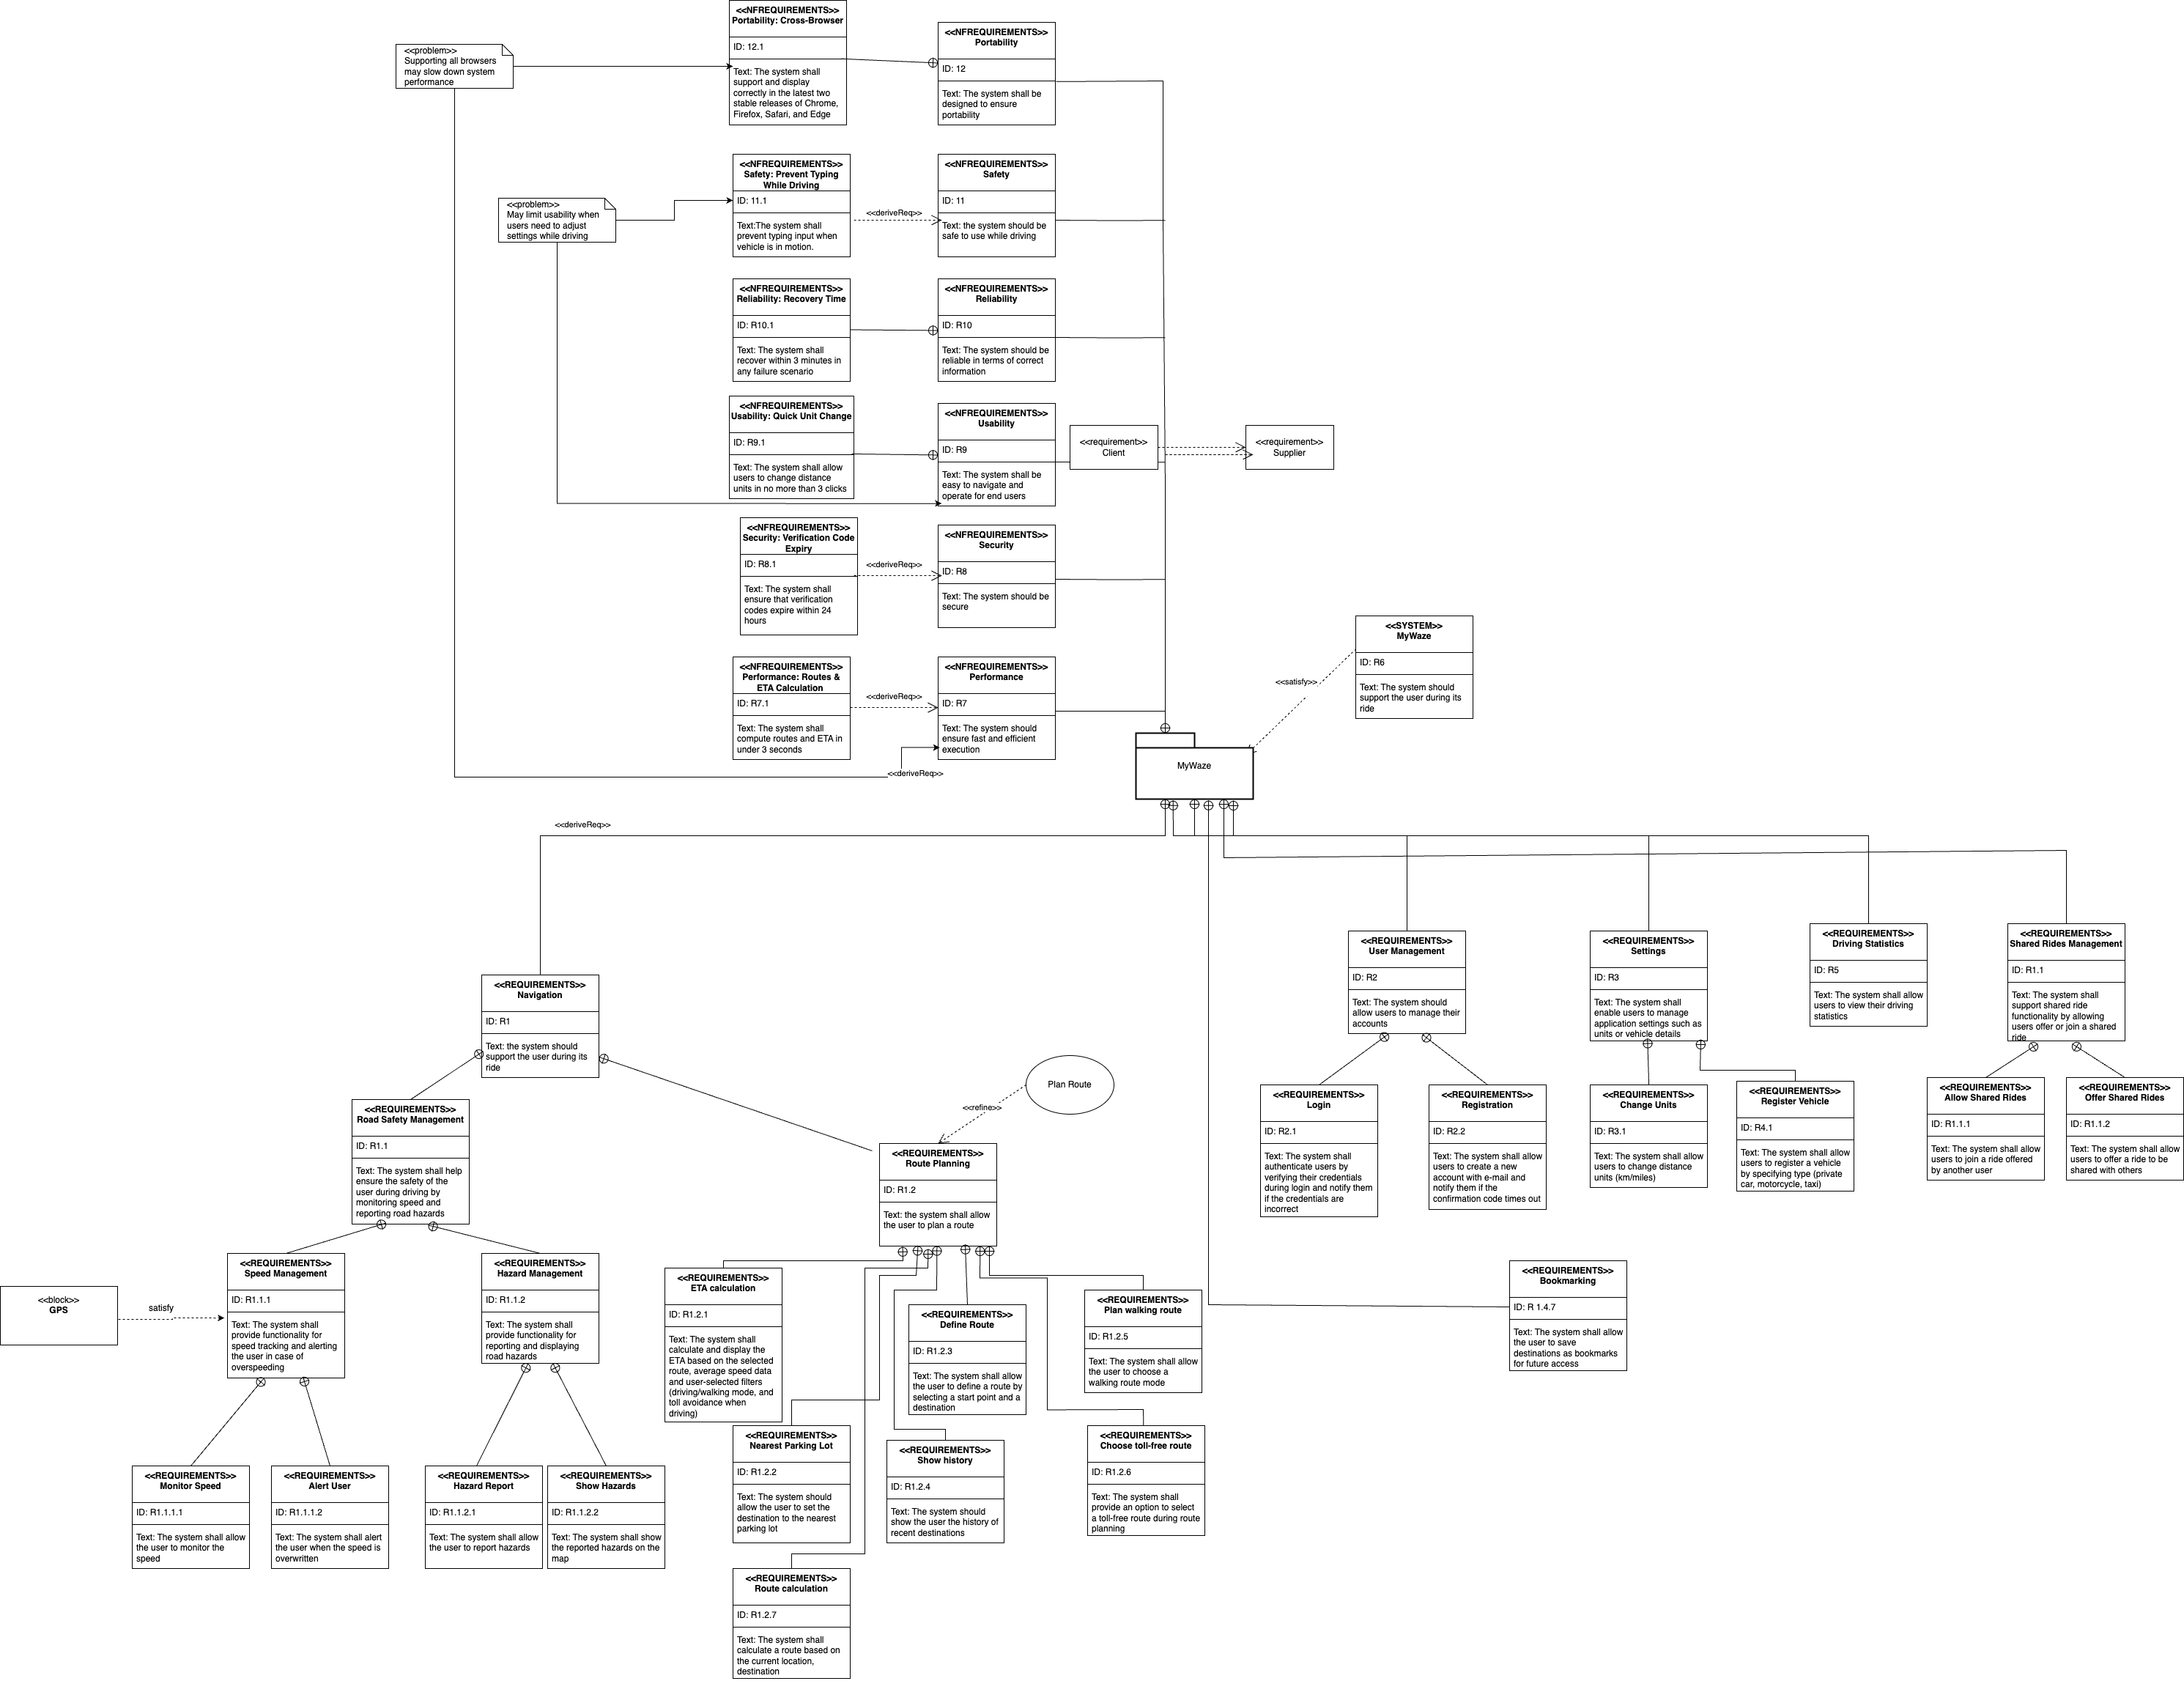
\includegraphics[width=\textwidth]{images/SysML_Req.png}
    \caption{Requirements Diagram}
    \label{fig:requirements_diagram}
\end{figure}

\clearpage

\section*{BPMN Models}

\modelentry{MyWaze}
\modelentry{MyWaze_ChangeUnit}
\modelentry{MyWaze_arrangeSharedRide}
\modelentry{MyWaze_calculateRoute}
\modelentry{MyWaze_createBookmark}
\modelentry{MyWaze_defineDestination}
\modelentry{MyWaze_defineRoute}
\modelentry{MyWaze_defineRouteToParkingLot}
\modelentry{MyWaze_navigate}
\modelentry{MyWaze_provideStatistics}
\modelentry{MyWaze_registerAccount}
\modelentry{MyWaze_registerRideOffering}
\modelentry{MyWaze_registerVehicleType}
\modelentry{MyWaze_reportHazard}
\modelentry{MyWaze_speedMonitoring}


\clearpage

\section*{Prototype}
\subsection*{Running Instructions}

\begin{lstlisting}[language=bash]
cd msp-mywaze-backend
npm i
npm run dev
\end{lstlisting}

\begin{lstlisting}[language=bash]
cd msp-mywaze-frontend
npm i
npm run dev
\end{lstlisting}

The only prerequisites are a current version of \texttt{node} and \texttt{npm}. The database is implemented as SQLite, so no manual setup is necessary.

Routing uses OpenRouteService, which is quota-limited (daily) in the free version. If it stops working, please wait one day or change the variable \texttt{ORS\_API\_KEY} in \texttt{msp-mywaze-backend/src/routes/routing.ts} to your own (free) API key obtained from \url{https://openrouteservice.org}.

\subsection*{Features Implemented}

\begin{itemize}
    \item \textbf{Registration}: User can register and login on home page.\\[0.5em]
    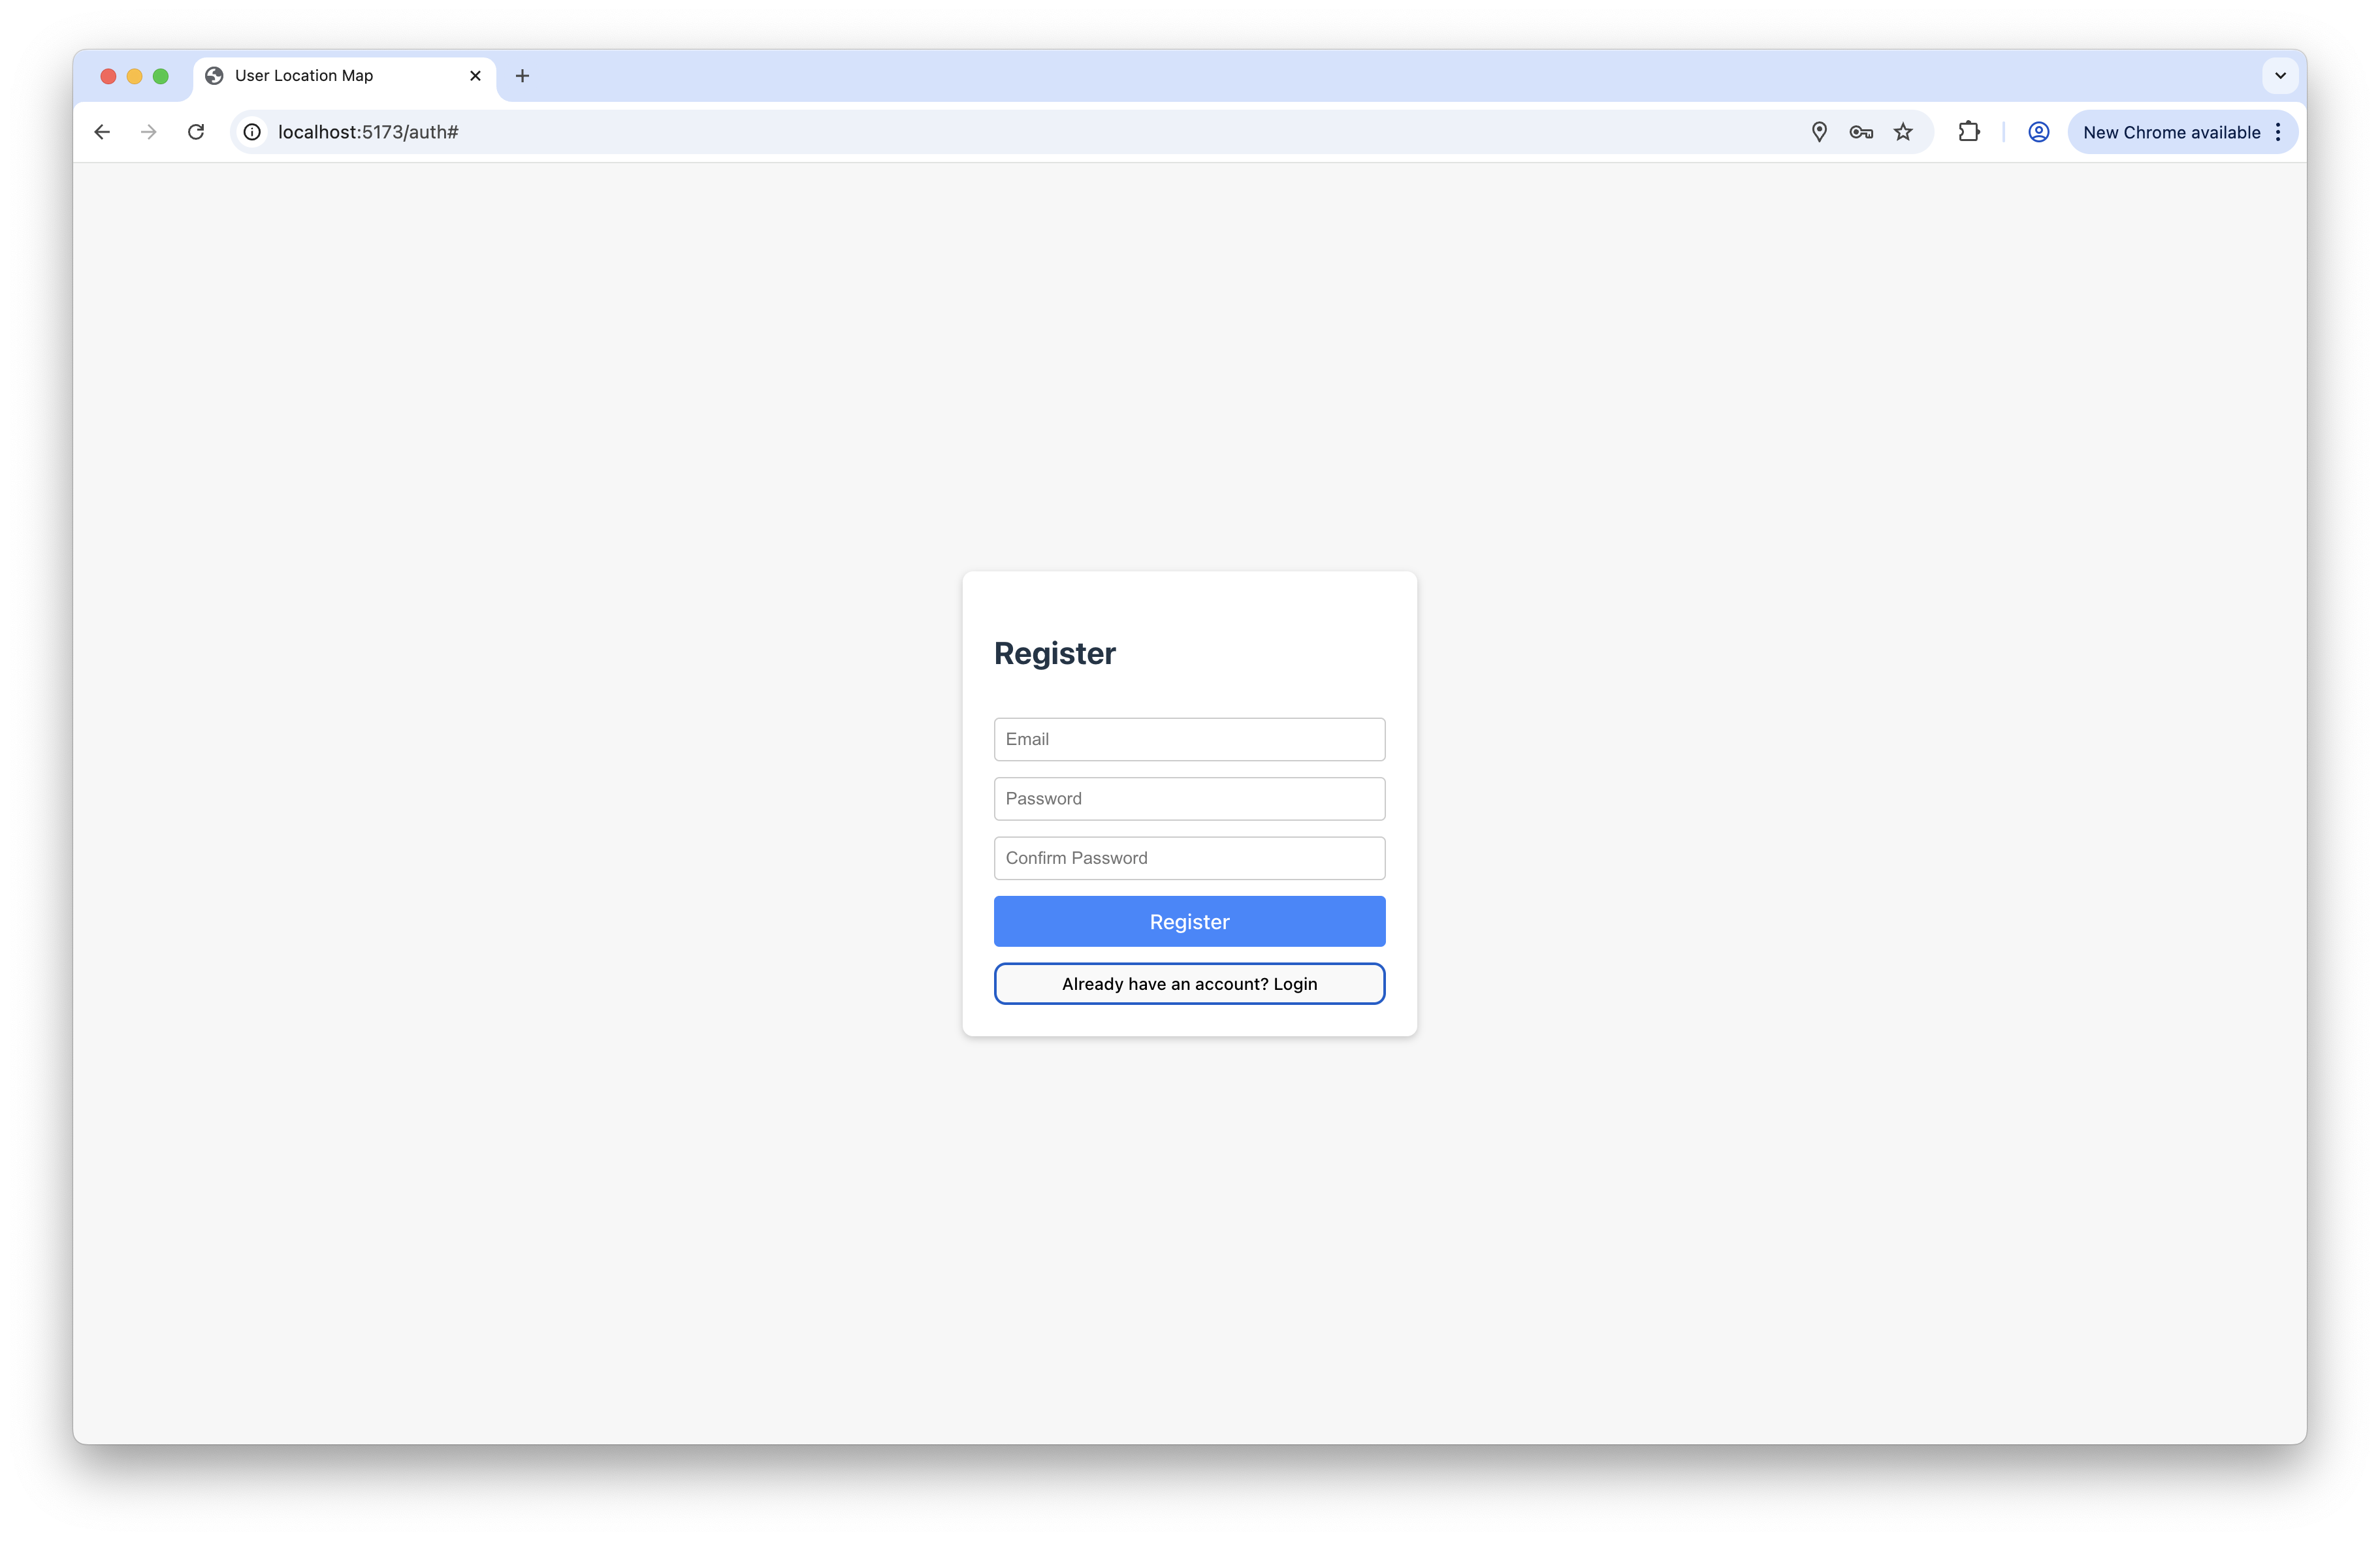
\includegraphics[width=\textwidth]{images/Registration.png}

    \item \textbf{Vehicle Type Registration}: User can configure their vehicle type in the drop-down user menu on the top right of the screen.

    \item \textbf{Define Route}: User can define a route by entering the destination name or address into the text field at the top center and clicking \textit{Go}.

    \item \textbf{ETA}: ETA is displayed in a popup above the destination after a route is defined.

    \item \textbf{Speed Warning}: Current speed will turn red if the user moves over 50 km/h. To test speed warnings on desktop, click on the speed value to generate a random speed around 50 km/h.\\[0.5em]
    \includegraphics[width=\textwidth]{images/Route_VehicleType_ETA_Speed.png}
\end{itemize}

\end{document}